\section{Návrh a analýza finální geometrie} \label{sec:finalni-geometrie}
    \subsection{Návrh konstrukčních úprav}
        Změny v rámci konstrukce sondy se týkaly zejména rozměrů trubic a odvětrání čidla\,A. Vzhledem k malému přínosu přidání difuzoru nebo kavit nebyly tyto konstrukční úpravy ve finální verzi sondy implementovány. Zachována byla trubice tvořící tělo sondy (rozměr $4 \times 0.4 \Unit{mm}$) a těsnění na koncích teplotních čidel. Čelo snímače B bylo posunuto na stejnou úroveň, jako čelo čidla\,A. 
        
        Stínící trubice čidla A byla zvětšena na rozměr $5 \times 0.5 \Unit{mm}$ a odvětrání bylo posunuto na $18 \Unit{mm}$ od čela stínění. Odvětrávací otvory byly zmenšeny na průměr $0.5 \Unit{mm}$ a byl zvýšen jejich počet ze $2$ na $4$, rozmístěny byly rovnoměrně po obvodu stínění.

        Čidlo B bylo, jako v kapitolách \ref{sec:sonda-se-stinenim-B} a \ref{sec:sonda-s-rozsirenym-stinenim-B}, opatřeno stíněním, v tomto případě tvořeném trubicí o rozměrech $9 \times 0.5 \Unit{mm}$, které bylo na koncích společně s trubicí uchycující čidlo B opatřeno zkosením $5^o$. Detailní rozměry modelu jsou uvedeny v příloze \ref{fig:sonda-final-vykres}.

        Potřebný měricí prostor se zvětšil z rozměru $37.5 \times 9 \times 4$ na $31 \times 14 \times 9$ ($x \times y \times z$), viz obrázek \ref{fig:sonda-final-porovnani}.

        \begin{figure}[ht!]
            \centering
            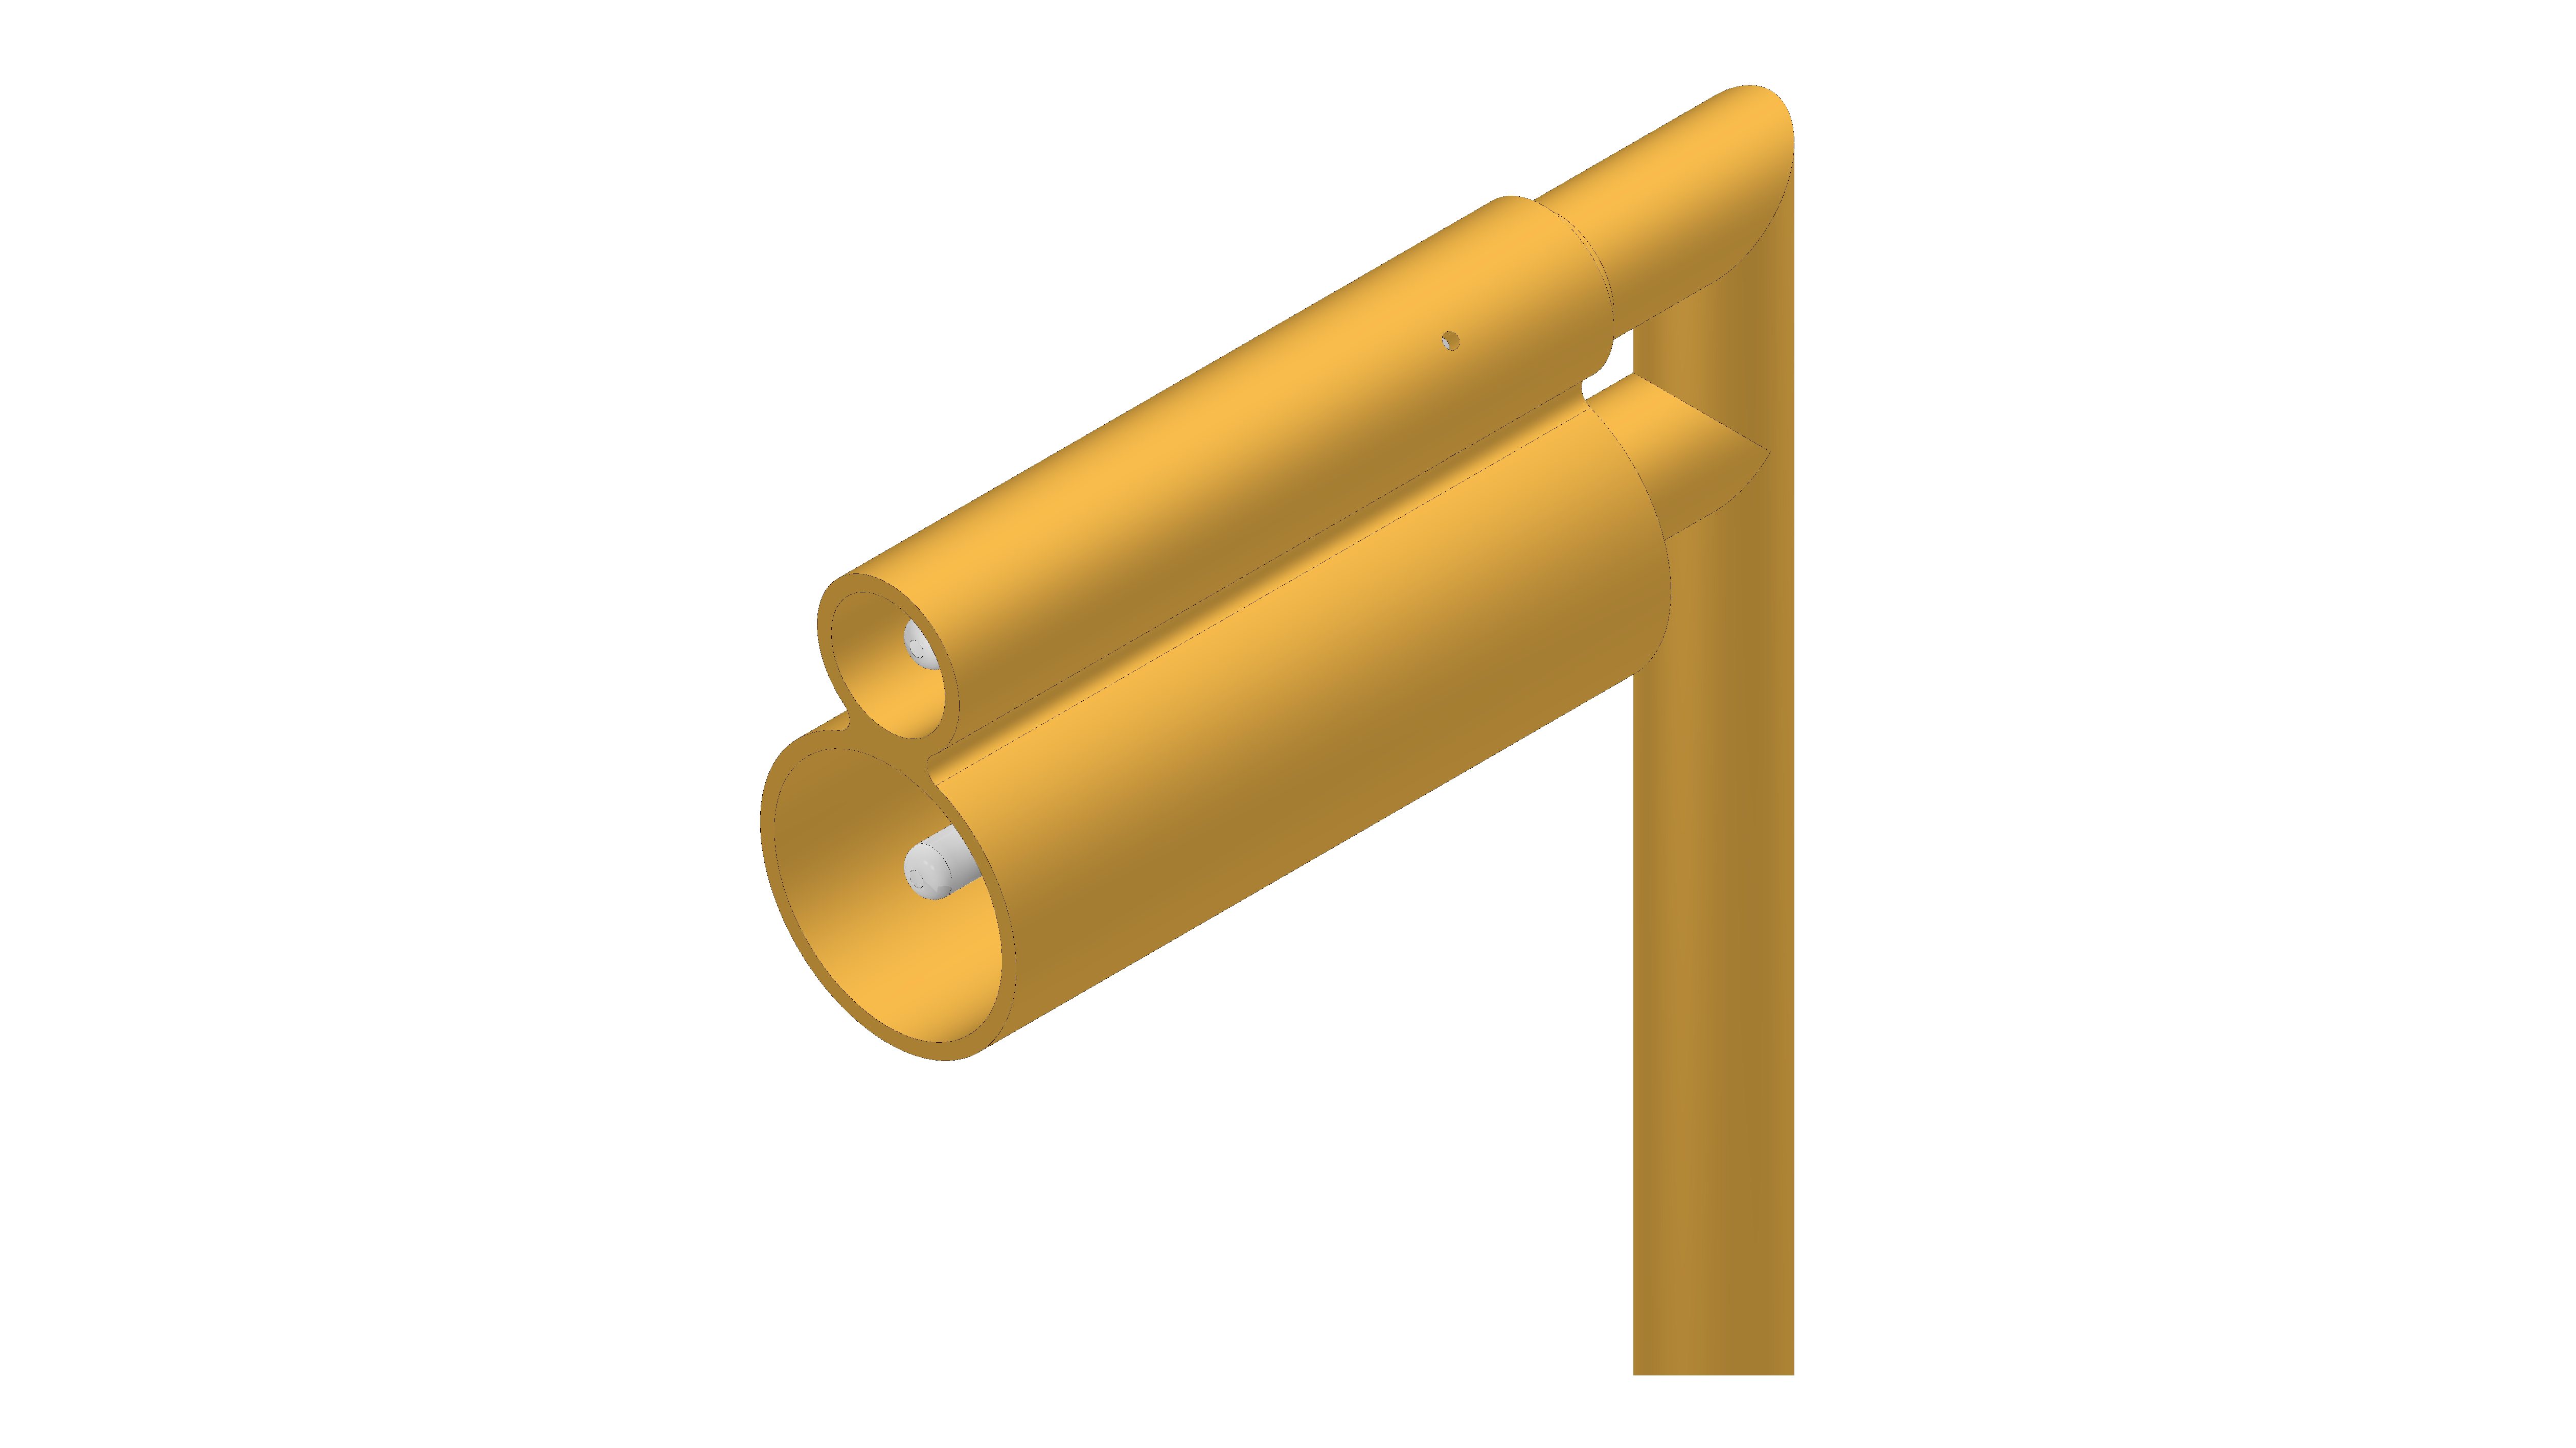
\includegraphics[width=\textwidth]{500_FINAL/sonda_final.png}
            \caption{Finální model DRTA sondy.}
            \label{fig:sonda-final}
        \end{figure}

        

        \begin{figure}[ht!]
            \centering
            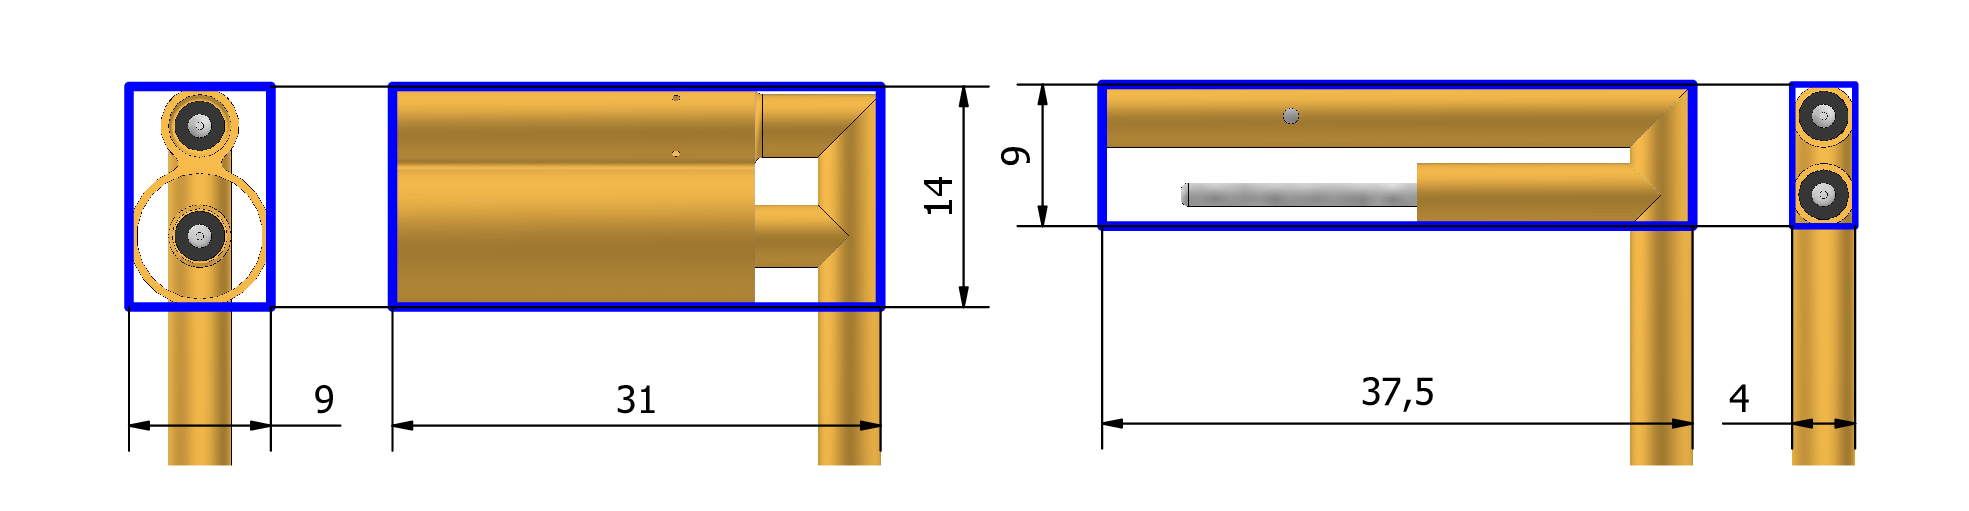
\includegraphics[width=\textwidth]{500_FINAL/porovnani_v01_final.png}
            \caption{Porovnání rozměrů finální (vlevo) a původní (vpravo) verze sondy.}
            \label{fig:sonda-final-porovnani}
        \end{figure}
        
    \subsection{CFD analýza}
        Chování restitučních faktorů bylo analyzováno stejným postupem, jako v kapitolách \ref{sec:sonda-bez-stineni-B} a \ref{sec:sonda-s-rozsirenym-stinenim-B} – byla zkoumána jejich závislost na rychlosti proudění ($100 \div 325 \Unit{\frac{m}{s}}$ ) a na natočení v rovině symetrie a kolmo na ní (v rozmezí $\pm 15^o$). Nakonec byl zkoumán vliv materiálu trubice, kde byla mosaz nahrazena ocelí a poté polykarbonátem.
        \subsubsection{Chování při různých rychlostech proudění}
            Přidané stínění k čidlu B zajistilo částečné vyrovnání průběhu rozdílu restitučních faktorů, což je nejvíce patrné pro rychlosti proudění do $225 \Unit{\frac{m}{s}}$, viz obrázek \ref{fig:sonda-final-rychlosti}. Při dalším zvyšování Machova čísla docházelo k poklesu rozdílu až na $92 \Unit{\%}$ hodnoty odpovídající rychlosti $250 \Unit{\frac{m}{s}}$, která byla rovna $0.1232$. 
            \begin{figure}[ht!]
                \centering
                \includegraphics*[width=\textwidth, trim={5.9cm 1.0cm 2.7cm 2.0cm}]{500_FINAL/final_rychlosti.eps}
                \caption{Závislost restitučních faktorů upravené sondy na rychlosti proudění.}
                \label{fig:sonda-final-rychlosti}
            \end{figure}

            Restituční faktor čidla A vzrostl v průměru o přibližně $2.03 \Unit{\%}$, nárůst u čidla B byl $1.76 \Unit{\%}$ pro rychlost $250 \Unit{\frac{m}{s}}$ a $2.54 \Unit{\%}$ pro rychlost $325 \Unit{\frac{m}{s}}$. Při nejnižší zkoumané rychlosti restituční faktor poklesl o $1.33 \Unit{\%}$, došlo tedy ke zlepšení jeho výsledného průběhu (přiblížení k \uv{rovnoběžným} průběhům), což se promítlo do již zmíněného vyrovnání rozdílu restitučních faktorů.

            \begin{figure}[ht!]
                \centering
                \begin{subfigure}{0.45\textwidth}
                    \centering
                    \captionsetup{width=.9\linewidth}
                    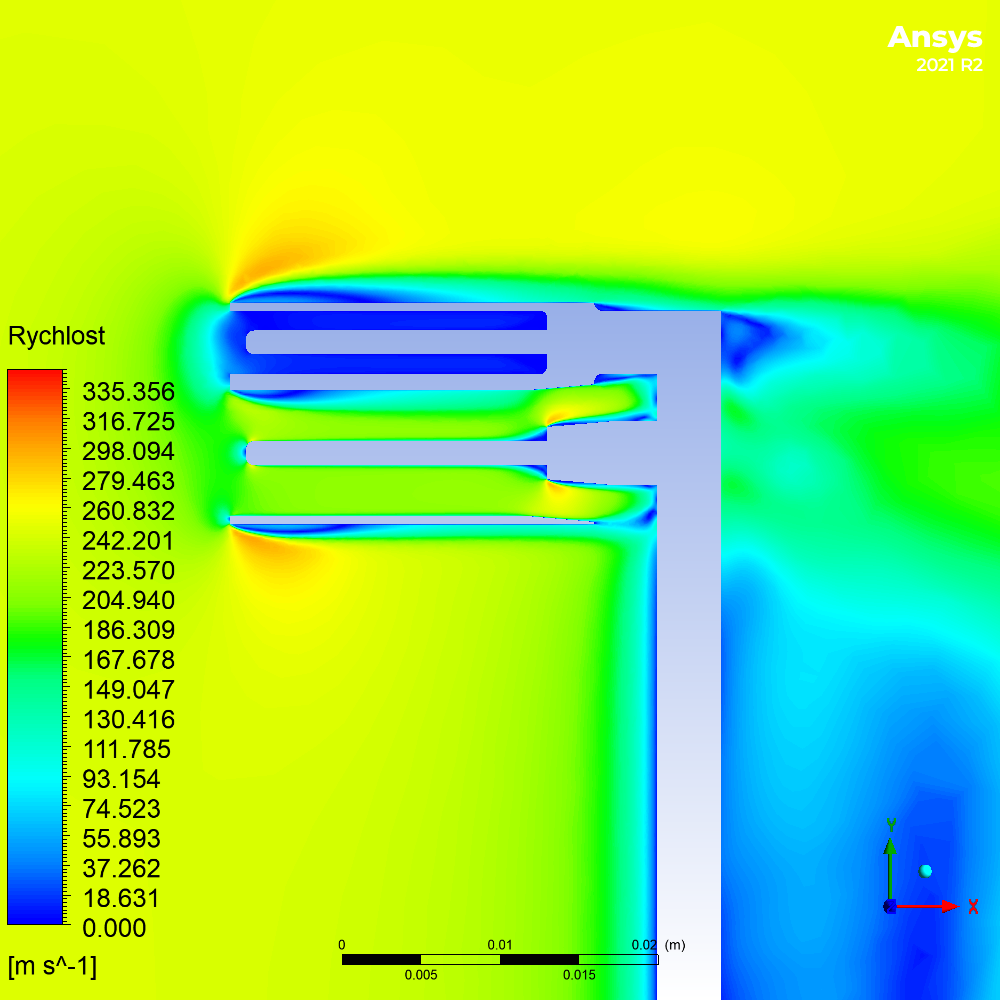
\includegraphics[width=\textwidth]{500_FINAL/SIM_Final_XY0_rychlost.png}
                    \caption{Rychlostní pole.}
                \end{subfigure}
                \begin{subfigure}{0.45\textwidth}
                    \centering
                    \captionsetup{width=.9\linewidth}
                    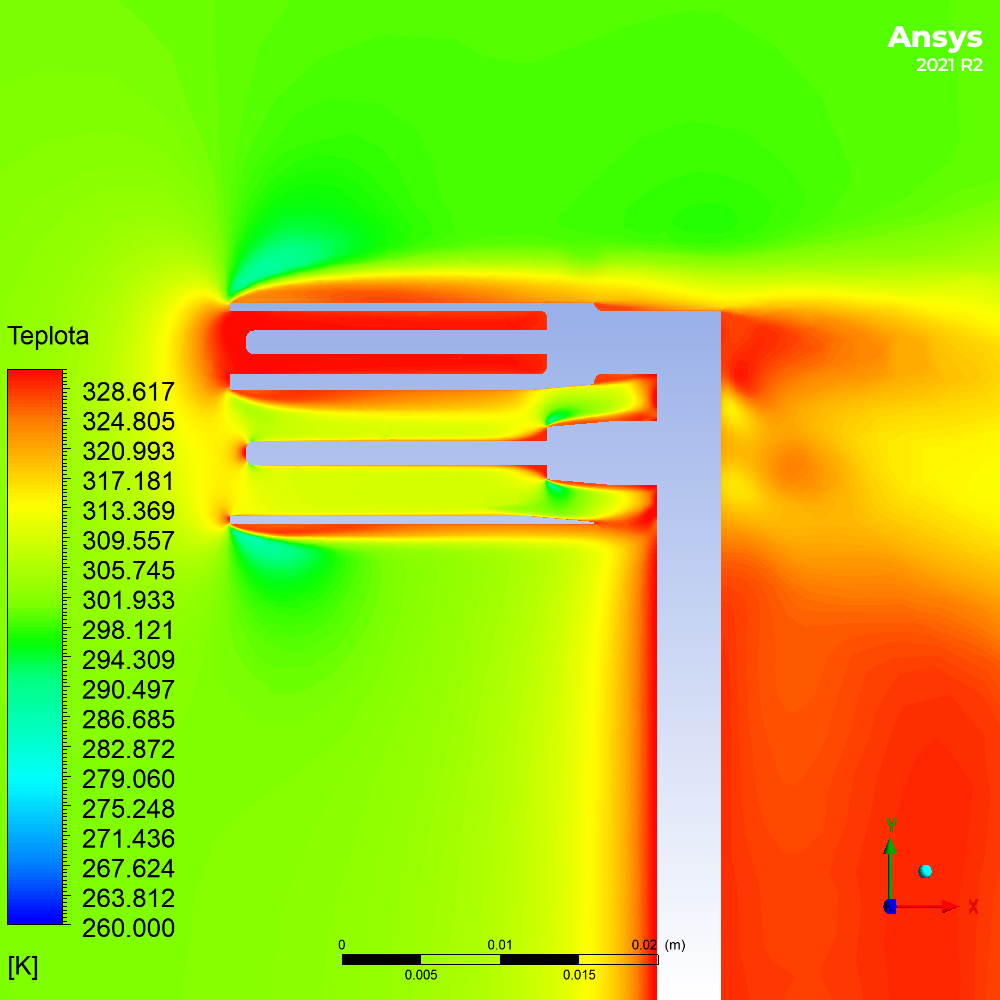
\includegraphics[width=\textwidth]{500_FINAL/SIM_Final_XY0_teplota.png}
                    \caption{Teplotní pole.}
                \end{subfigure}
                \caption{Vizualizace vypočtených dat pro upravenou sondu v rovině symetrie pro rychlost proudění $250 \Unit{\frac{m}{s}}$.}
                \label{fig:sonda-final-vizualizace}
            \end{figure}

        \newpage
        \subsubsection{Směrová citlivost v rovině symetrie}
            \begin{figure}[ht!]
                \centering
                \includegraphics*[width=\textwidth, trim={5.9cm 1.0cm 2.7cm 2.0cm}]{500_FINAL/final_XY.eps}
                \caption{Závislost restitučních faktorů upravené sondy na natočení v rovině symetrie.}
                \label{fig:sonda-final-symetrie}
            \end{figure}
        \subsubsection{Směrová citlivost kolmo na rovinu symetrie}
            \begin{figure}[ht!]
                \centering
                \includegraphics*[width=\textwidth, trim={5.9cm 1.0cm 2.7cm 2.0cm}]{500_FINAL/final_XZ.eps}
                \caption{Závislost restitučních faktorů upravené sondy na natočení kolmo na rovinu symetrie.}
                \label{fig:sonda-final-kolma-rovina}
            \end{figure}
        \subsubsection{Volba materiálu trubice}

        \subsubsection{Zhodnocení}

            \begin{figure}[ht!]
                \centering
                \includegraphics*[width=\textwidth, trim={0.0cm 1.0cm 1.0cm 0.0cm}]{500_FINAL/final_rozdil_restitucnich_faktoru.eps}
                \caption{Porovnání závislostí rozdílu restitučních faktorů s vyznačením $2.5\%$ ,$5\%$ a $10\%$\,odchylky od hodnoty v nevychýleném stavu a při rychlosti proudění $250 \Unit{\frac{m}{s}}$.}
                \label{fig:sonda-final-rozdil-restitucnich-faktoru}
            \end{figure}

            \begin{figure}[ht!]
                \centering
                \includegraphics*[width=\textwidth, trim={5.9cm 1.0cm 2.7cm 2.0cm}]{500_FINAL/final_chyba_mereni.eps}
                \caption{Rozložení chyb měření rychlosti při uvažování konstantního rozdílu restitučních faktorů.}
                \label{fig:sonda-final-chyba-mereni}
            \end{figure}


        
        